\chapter{Contrast Improvement of Neutron Interferometry Measurements} % Write in your own chapter title
\label{Chapter2}
\lhead{Chapter 2. \emph{Contrast Improvement of Neutron Interferometry Measurements}} % Write in your own chapter title to set the page header

\section{Bayesian Markov Chain Monte Carlo Algorithms}
Ever since Max Born presented what would become to be known as the Born interpretation, quantum mechanics has become a science of probabilities. The Born rule states that the probability of measuring an eigenvalue $\lambda_i$  of an observable corresponding to a hermitian operator $A$  will be 
\begin{equation}
p(\lambda_i) = \Braket{\Psi|P_i|\Psi}
\label{eq:bornrule}
\end{equation}
This can be seen by applying the spectral theorem to $A$\cite{linear}
\begin{equation}
A = \lambda_1 P_1 + \lambda_2 P_2 \cdots \lambda_i P_i
\end{equation}
Where $P_i$ are the orthogonal projections of $A$ onto the eigenspace corresponding to $\lambda_i$. As $I = P_1 + P_2 \cdots + P_i$ and $\Braket{\Psi|\Psi} = 1$ given a probabilistic interpretation of the inner product. 
\begin{equation}
\Braket{\Psi|I|\Psi} =\Braket{\Psi|P_1|\Psi} + \Braket{\Psi|P_2|\Psi} + \cdots +\Braket{\Psi|P_i|\Psi}  = 1
\end{equation}
Given this result the interpretation may be made that 
\begin{equation}
\Braket{\Psi|A|\Psi} = \lambda_1 \Braket{\Psi|P_1|\Psi} + \lambda_2\Braket{\Psi|P_2|\Psi} + \cdots +\lambda_i\Braket{\Psi|P_i|\Psi} =\lambda_1 p(\lambda_1) + \lambda_2p(\lambda_2) + \cdots +\lambda_ip(\lambda_i) = \bar{\lambda} 
\label{eq:quantumExpectation}
\end{equation}
Therefore it is quite easy to see where the Born rule arises. It is therefore clear that the Born interpretation opens physics up to the world of statisticians and their probabilities. Using techniques from statistics it is possible that improvements in neutron interferometer contrast may be made. 
\subsection{Baye's Theorem} 
Baye's theorem is a very interesting statistical method that is useful for predicting the accuracy of statistical models given event data. The generic form of Baye's Thereom is 
\begin{equation}
P(A|B) = \frac{P(B|A)P(A)}{P(B)} 
\label{eq:bayes}
\end{equation}
What this says is that given an event $B$ occurring from a set of events $\mathcal{E}$, the posterior probability that the model $A$ describing it is the most likely model in the set of models $\mathcal{M}$ is the probability of event $B$ occurring according to model $A$ multiplied by the prior likelihood of model $A$ and normalized by the total probability of event $B$ occurring according to all models in set $\mathcal{M}$.\cite{bayes}

This is an incredibly powerful theorem as it allows a set of models to be analysed statistically to determine the correct model with an actual likelihood of correctness given event data. A broad range of models can be tested and as more data rolls in the likelihood of the correct model to describe the system will rise.

There are discrete and continuous forms of Baye's theorem, however in this case only the discrete form is of interest. 
\begin{equation}
P(A_i|B) = \frac{P(B|A_i)P(A_i)}{\sum \limits_j P(B|A_j)P(A_j)}
\label{eq:discretebayes}
\end{equation}
\begin{figure}[ht!]
\centering
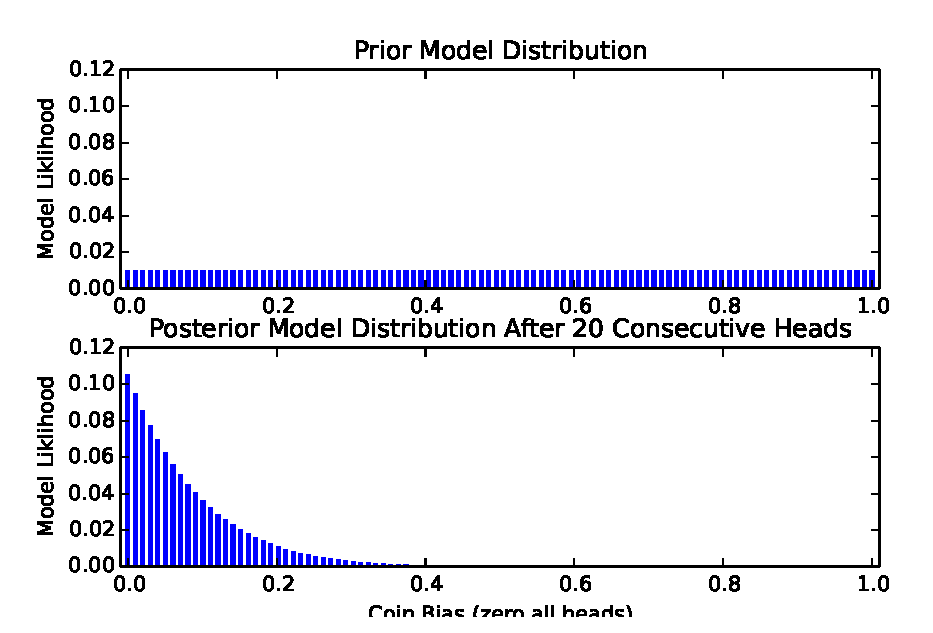
\includegraphics[scale=0.5]{Figures/bayes.eps}
\caption{Example prior and posterior distribution for a set of coin flip models that samples 10 heads flips in a row}
\label{fig:bayes}
\end{figure}
\subsection{Markov Chain Monte Carlo Methods}
Often when attempting to fit a model it is computationally infeasible to explore the entire model space. This can be due to having a large number of possible models, models having a large number of parameters and the fact that most physical process parameters are described by real numbers and it is therefore impossible to explore the entire parameter space. A way to deal with model selection in this case is known are Markov Chain Monte Carlo (MCMC) methods. Given a set of models 
\begin{equation}
\mathcal{M} = \left\{\mathbf{M}(x_1,x_2,\cdots,x_i;y_1,y_2,\cdots,y_i) : y_j \in \mathcal{F}\right\}
\label{eq:models}
\end{equation}
where $x_j$ are input variables to the model and $y_j$ are model parameters, it is desired to find and approximate ideal model. MCMC methods will select an original set of possible model parameters $$\mathbf{P} = \left\{(y_{11},y_{12},\cdots,y_{1i}),\cdots,(y_{j1},y_{j2},\cdots,y_{ji})\right\}$$ and assign a prior distribution to these models $\mathcal{D}_{prior}$. Given a set of inputs $$\mathbf{I} = \left\{(x_{11},x_{12},\cdots,x_{1i}),\cdots,(x_{j1},x_{j2},\cdots,x_{ji})\right\}$$ the posterior distribution $\mathcal{D}_{pos}$ can be evaluated using (\ref{eq:discretebayes}). In order to explore the parameter space, the algorithm must select a new set of parameters. One method of doing this is to select some $\subset \mathbf{P}$ and generate a new set of models and posterior distributions according to some utility function\cite{bayes}
\begin{equation}
\mathcal{M}_{pos},\mathcal{D}_{pos_2} = f(\mathcal{M},\mathcal{D}_{pos})
\label{mcmcupdate} 
\end{equation}

It is useful to think of the set of selected model parameters as a large number of points in space, in practice these are often referred to as points. By re-sampling model parameters as in (\ref{mcmcupdate}) it is possible to select points throughout the parameter space and ideally zero in on the optimal model. However, due to the nature of sampling normally being non-deterministic and numerical precision errors, it is crucial examine the convergence of the model to experimental data. 

\subsection{Fisher Information and the Cramer-Rao Lower Bound}
The Cramer-Rao lower bound is hugely important in statistics as it provides a lower bound on the variance of an unbiased estimator 
\subsubsection{Covariance Matrix}
The covariance matrix in statistics is a measure of how a random vector of variables changes together. Two random variables are related by their covariance $\sigma(x,y) = E_x \left[(x-E[x])(y-E[y])\right]$, where $E[x]$ denotes the expectation value of $x$. As an example, in quantum mechanics the expectation value according to the Born interpretation is as in (\ref{eq:quantumExpectation}). The covariance of two random variables can be generalized to that of a random vector of estimated coefficients $\mathbf{X}$ where \cite{covariance}
\begin{equation}
cov(\mathbf{X})_{ij} = cov(X_i,X_j) = E[(X_i-E[X_i])(X_j-E[X_j])]
\end{equation}
Which in matrix notation takes the form 
\begin{equation}
cov(\mathbf{X}) = [(\mathbf{X}- u)(\mathbf{X}-u)^T] = E(\mathbf{X}\mathbf{X}^T) - uu^T
\label{eq:covarianceMatrix}
\end{equation}
Where $u=E(\mathbf{X})$. It is prudent to note that the elements of the diagonal of the covariant matrix $\sum{ii}$ are the variances of the elements of the vector $\mathbf{X}$. When $\sigma(x,y)>0$ the relationship between the two variables tends to be similar, ie. when one grows the other grows and similarly when $\sigma(x,y)<0$ when one variable grows the other will tend to show the opposite behaviour.\cite{covariance}  

\subsubsection{Cramer-Rao Lower Bound}
The Cramer-Rao lower bound states that the variance of an unbiased estimator $\hat{\theta}$ is lower bounded by the reciprocal Fisher Information $I(\theta)$.\cite{cramer} 
\begin{equation}
var(\hat{\theta}) \geq \frac{1}{I(\theta)}
\label{cramerao}
\end{equation}
The Fisher Information is the expectation value of the square of the first moment of the log likelihood function for some probability density function $p(\mathbf{X};\theta)$. The log-likelihood of the probability density function is defined as $\mathcal{l}(\mathbf{X};\theta) = log(p(\mathbf{X};\theta))$
Therefore the Fisher information is 
\begin{equation}
I(\theta) = E\left[\left(\frac{\partial}{\partial \theta} log (p(\mathbf{X};\theta)) \right)^2 \Big| \theta \right] = -E\left[\frac{\partial^2}{\partial\theta^2} l(\mathbf{X};\theta) \Big| \theta \right]
\label{fisherinformation}
\end{equation}
The Fisher Information is the variance of the statistical score of the probability density function. Geometrically it is a measure of the amount of curvature of the log-likelihood function. It is a measure of the amount of information an observable $\mathbf{X}$ carries about an unknown parameter $\theta$ of which the probability of $\mathbf{X}$ relies on according to the function $p(\mathbf{X};\theta)$. 

The Cramer-Rao lower bound establishes a lower limit on the amount of information an unknown parameter of a probability distribution carries.\cite{cramerrao2} This is very useful in determining the fit of a set of model parameters as shall be seen. It is important to keep in mind that this only holds for unbiased estimators and may be violated by biased estimators. 
\section{Q-Infer}
\subsection{Interaction with NI-Engine}
\subsection{GPU Implementations of Likelihood functions}